\section{Decay-Candidate Selection and Background}
\label{sec:ana_bkgSub}
%show mass-fit results in $\cthetal$ bins

While the decay model discussed in Chapter~\ref{chap:pheno} describes the \BstoJpsiKK{} signal, the time and angular distribution in the
experimental data contains both signal and background decay candidates. The background distribution is subtracted from the total
distribution in the data to be able to fit the model to the signal distribution. Since there are statistical uncertainties associated to
both the total distribution and the subtracted background distribution, however, the resulting uncertainties in the signal-parameter
estimates become larger with an increasing amount of background decay candidates. Therefore, a selection procedure is applied, designed to
reject as many background candidates as possible without removing too many signal candidates.


%%%%%%%%%%%%%%%%%%%%%%%%%%
\subsection{Selection}
\label{sec:ana_bkgSub_sel}
%%%%%%%%%%%%%%%%%%%%%%%%%%

The decay-candidate selection procedure is briefly described here. See reference~\cite{Aaij:2014} for a detailed discussion.

As described in Section~\ref{subsec:intro_LHCb_Jpsiphi}, the first selection requirements are applied in the L0 trigger, which only selects
events with hits in the LHCb muon stations and particles with a sufficiently high (transverse) momentum. From the events that remain, the
HLT reconstructs and selects $\mumu$ pairs that are likely to originate from a $\Jpsi\to\mumu$ decay. Offline, the resulting
$\Jpsi\to\mumu$ candidates are matched to $\KK$ pairs to form \BstoJpsiKK{} decay candidates. The four tracks these candidates consist of
are required to be compatible with a $\Bs$ that was produced in the associated primary vertex and decayed at a decay time above a given
threshold.

In both HLT1 and HLT2 there are two different types of selections applied. The first type does not use any information on the distance that
the $\Bs$ travelled before it decayed and the second type does. Requiring a minimum flight distance reduces the fraction of
background candidates significantly, since all four tracks originate from the primary vertex for most combinatorial background, while the
tracks in a $\Bs$ decay originate from a secondary vertex at some distance from the primary vertex. However, the flight distance variable
is correlated with the decay time variable and requiring a minimum flight distance introduces a non-trivial selection efficiency as a
function of decay time. Therefore, the sets of selection criteria that use information on the flight distance are called \emph{decay-time
biasing} or \emph{biased}.

The unbiased HLT1 selection requires two oppositely charged muon candidates that are close enough to originate from one decay vertex and
have a $\mumu$ invariant mass greater than 2.7\unitsp\GeV. The biased HLT1 selection does not require a $\Jpsi$ candidate, but selects
single tracks with a perpendicular distance to any primary vertex greater than 0.1\unitsp{}mm. Both of these selections reduce the number
of selected events to a manageable level. Approximately 68\% of the decay candidates that are finally used in the fit is selected by both
the unbiased and biased selections, approximately 14\% exclusively by the unbiased selection, and approximately 19\% exclusively by the
biased selection.
% HLT1: 81% unbiased; about the same numbers for the signal

Both the unbiased and the biased HLT2 selections require $\Jpsi\to\mumu$ candidates with an invariant $\mumu$-mass within a window of
0.24\unitsp\GeV{} centred at the $\Jpsi$ mass of 3.10\unitsp\GeV. In addition, the biased selection requires a minimum \emph{decay-length
significance} (DLS) of three for the $\Jpsi$ candidate. The DLS is defined as the distance between the $\mumu$ vertex and the associated
primary vertex (\emph{decay length}) divided by the uncertainty on this distance. Since the decay length is a measure of the flight
distance of the $\Bs$, this requirement is decay-time biasing.

Without the minimum-DLS requirement the rate of events that pass the HLT2 selection would be too high to handle online. Therefore, the
rate of the unbiased selection is reduced by processing only a fraction of the events that pass the HLT1 selection. To keep the selection
unbiased, the processed events are randomly selected, without considering any information on the reconstructed particles. In the final
data sample that is used in the fit, the number of decay candidates that is exclusively selected by the unbiased HLT2 selection is three
per cent of the number of candidates selected by the biased selection. Considering only signal candidates, the unbiased HLT2 selection adds
one per cent to the total.

The method of modelling the non-trivial decay-time efficiency shape introduced by the biased HLT selections is discussed in
Section~\ref{subsec:ana_time_acc}. Because the unbiased HLT2 selection adds only few signal candidates to the final data sample, but
including these data complicates modelling of the efficiency significantly, only the time and angular distributions of HLT2-biased
candidates are fitted. However, candidates selected by the unbiased HLT2 selection are used to extract the efficiency shapes from the
\BstoJpsiKK{} data. The efficiencies of the biased selections are determined relative to the uniform efficiencies of the unbiased
selections. 

In the offline reconstruction process the muon tracks and the $\mumu$ vertex of $\Jpsi\to\mumu$ candidates selected by HLT2 are combined
into \BstoJpsiKK{} candidates with two oppositely charged kaons that form a $\KK$ vertex. The subsequent stripping selection imposes
requirements on how well detector hits form tracks within experimental uncertainties, how well tracks form $\mumu$, $\KK$, and $\mumu\,\KK$
vertices, the particle transverse momenta, the likelihood that the particles are identified correctly as muons and kaons, the invariant
masses of the reconstructed $\mumu$, $\KK$, and $\JpsiKK$ combinations, and the decay time of the candidate. About twelve million
\BstoJpsiKK{} candidates remain after this selection stage.

The selection of decay candidates is refined in the final offline stage. To visualize the effect of the selection, the distribution in
$\JpsiKK$ mass of remaining decay candidates is plotted for different selection requirements in Figure~\ref{fig:JpsiKKMassSel}. Notice that
the figure shows only a part of the mass range.
\begin{figure}[htb]
  \centering
  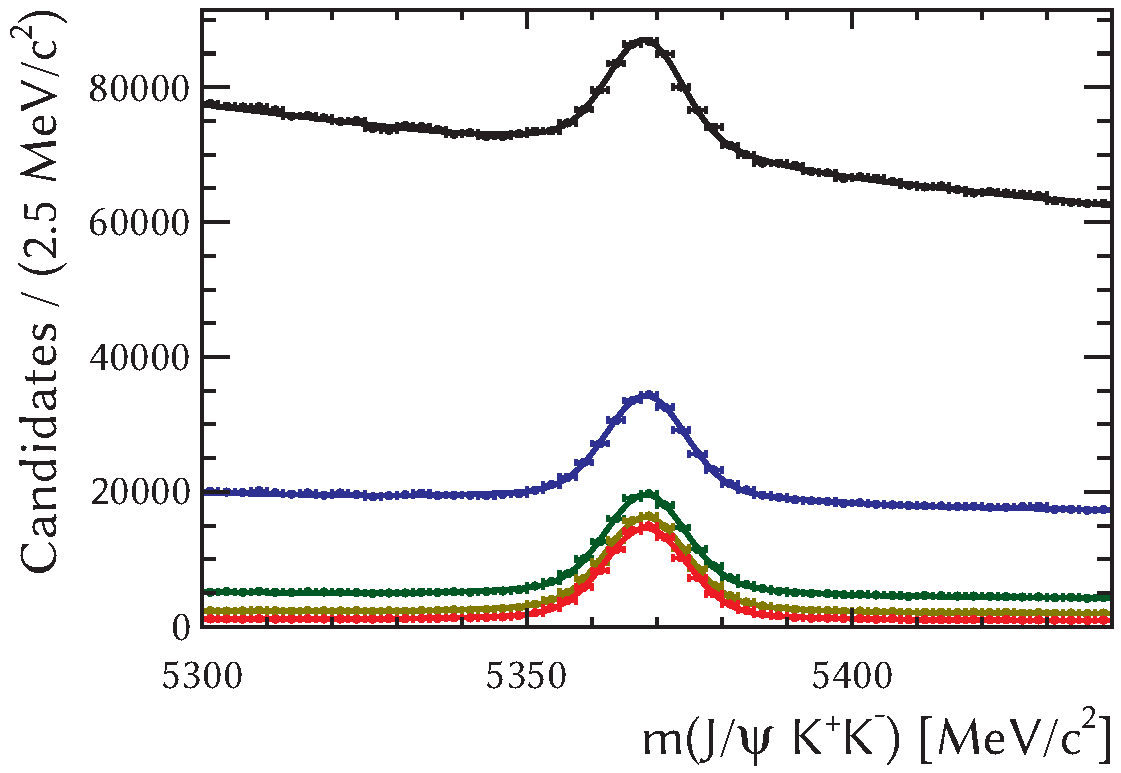
\includegraphics[width=0.7\textwidth]{graphics/analysis/JpsiKKMassSel}
  \caption{Distribution of \BstoJpsiKK{} decays in $\JpsiKK$ mass for different selection criteria.
           The data are shown as points, while the lines represent a model that consists of the sum of two Gaussian shapes (signal)
           and an exponential shape (combinatorial background).
           Subsequent selection criteria are applied in addition to previous criteria:
           black: stripping selection; blue: minimum quality of $\Bs$ decay-vertex reconstruction;
           green: minimum $\KK$ transverse momentum; yellow: minimum decay time; red: full offline selection.
           Notice that only a part of the total mass range is shown.}
  \label{fig:JpsiKKMassSel}
\end{figure}

For \BstoJpsiKK{} signal candidates this distribution is a peak around the value of the $\Bs$ mass of approximately 5367\unitsp\MeV. The
width of this peak is determined by the experimental resolution on the $\JpsiKK$-mass measurement. The background is mainly combinatorial
and follows an exponential distribution, which decays slowly across the considered mass range. Because of the obvious difference in
distributions of $\JpsiKK$ mass for the signal and the background, this variable can be used to statistically separate the two
contributions.

The distribution of black data points in Figure~\ref{fig:JpsiKKMassSel} is for candidates that pass the stripping selection without further
requirements. A peak of signal candidates is visible on top of a large background distribution. To determine the numbers of signal and
background candidates, the surface areas underneath the peak and the exponential distribution are determined with a fit. The signal peak is
modelled with the sum of two Gaussian shapes and the background with and exponential shape. The fit yields approximately 123 thousand
signal candidates, which corresponds to a signal fraction of approximately one per cent.

In the rest frame of the $\Bs$, the momentum of the $\KK$ pair is approximately 1.6\unitsp\GeVc{} for signal decays. Boosting into the
frame of the detector, approximately along the beam axis, this translates in a typical transverse momentum above 1\unitsp\GeVc. The sum of
the transverse momentum components of two kaons that accidentally form a suitable $\KK$ vertex in combinatorial background is often not
sufficient to make a transverse momentum of 1\unitsp\GeVc. As a result, requiring this value as a minimum in the offline selection removes
about 74\% of the background, but only 6\% of the signal, with respect to the stripping selection where already a minimum of
0.5\unitsp\GeVc{} was required. The $\JpsiKK$-mass distribution with the $\KK$ transverse momentum requirement is shown by the blue points
in Figure~\ref{fig:JpsiKKMassSel}.

To estimate the position of the $\Bs$ decay vertex and the kinematics of the particles in the decay as well as possible, these variables
are determined from a fit. The fit takes the position of the primary vertex, the muon and kaon tracks, and the corresponding experimental
uncertainties as inputs and minimizes a $\chi^2$ function for the position of the decay vertex and its perpendicular distance to the flight
path of the $\Bs$, which should be equal to zero. The value of the $\chi^2$ function in its minimum is a measure of the quality of the fit,
i.e. of how well the four reconstructed particles form a $\Bs$ decay vertex. The fit will in general be good for signal candidates, which
results in small values for the $\chi^2$ function.

Requiring a $\chi^2$ smaller than five times the number of degrees of freedom in the vertex fit removes about 75\% of the background that
remains after requiring a minimum $\KK$ transverse momentum of 1\unitsp\GeVc. Approximately 8\% of the remaining signal is lost. The
distribution of decay candidates after the $\KK$ transverse momentum and vertex fit quality requirements is shown by the green points in
Figure~\ref{fig:JpsiKKMassSel}.

A third requirement that removes a significant part of the background is a minimum on the reconstructed value of the decay time. For most
of the background candidates the four particles originate directly from the primary vertex, which corresponds to vanishing decay time
within experimental resolution. The stripping selection already requires a minimum decay time of 0.2\unitsp{}ps. Requiring a minimum of
0.3\unitsp{}ps in addition to the stripping selection and the $\KK$ transverse momentum and vertex fit $\chi^2$ requirements removes about
54\% of the remaining background and 6\% of the signal. The distribution for remaining candidates is shown by the yellow points in
Figure~\ref{fig:JpsiKKMassSel}.

Finally applying the full offline selection removes another 62\% of the background and 6\% of the signal, leaving approximately 94
thousand signal candidates and 135 thousand background candidates for further analysis. This corresponds to a signal fraction of 41\% in
the full $\JpsiKK$-mass range of 5200--5550\unitsp\MeV{} after the full selection. The final distribution is shown by the red points in
Figure~\ref{fig:JpsiKKMassSel}.

Notice, however, that the signal candidates are concentrated in a mass window of approximately 60\unitsp\MeV, centred at the $\Bs$ mass,
where the signal fraction is approximately 80\%. The regions to the left and the right of this \emph{signal window} are called mass
\emph{side bands} and contain only background candidates. The candidates in the side bands are used to estimate the time and angular
distribution of the combinatorial background and subtract this from the total distribution in the signal window to obtain the signal
distribution. This procedure is described in the following section.


%%%%%%%%%%%%%%%%%%%%%%%%%%%%%%%%%%%
\subsection{Background Subtraction}
\label{sec:ana_bkgSub_bkgSub}
%%%%%%%%%%%%%%%%%%%%%%%%%%%%%%%%%%%


\begin{figure}[htb]
  \centering
  \begin{subfigure}{0.49\textwidth}
    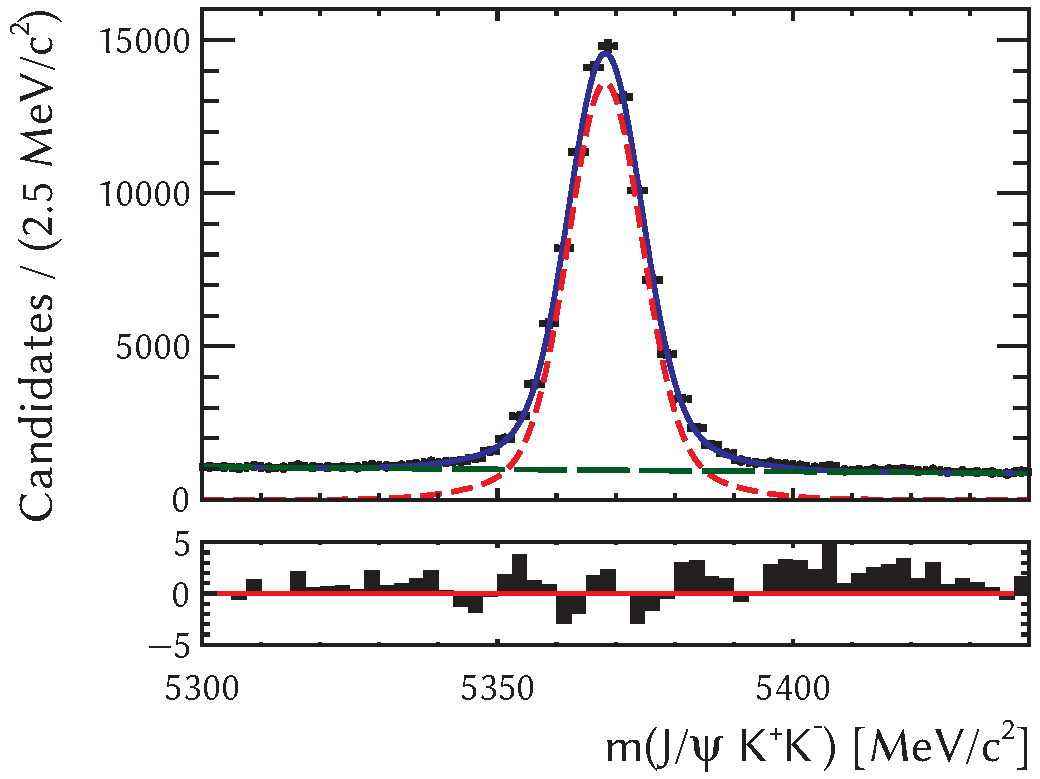
\includegraphics[width=\textwidth]{graphics/analysis/JpsiKKMass_DG_lin_resid}
    \caption{}
    \label{fig:JpsiKKMass_DG_lin}
  \end{subfigure}%
  \hfill%
  \begin{subfigure}{0.49\textwidth}
    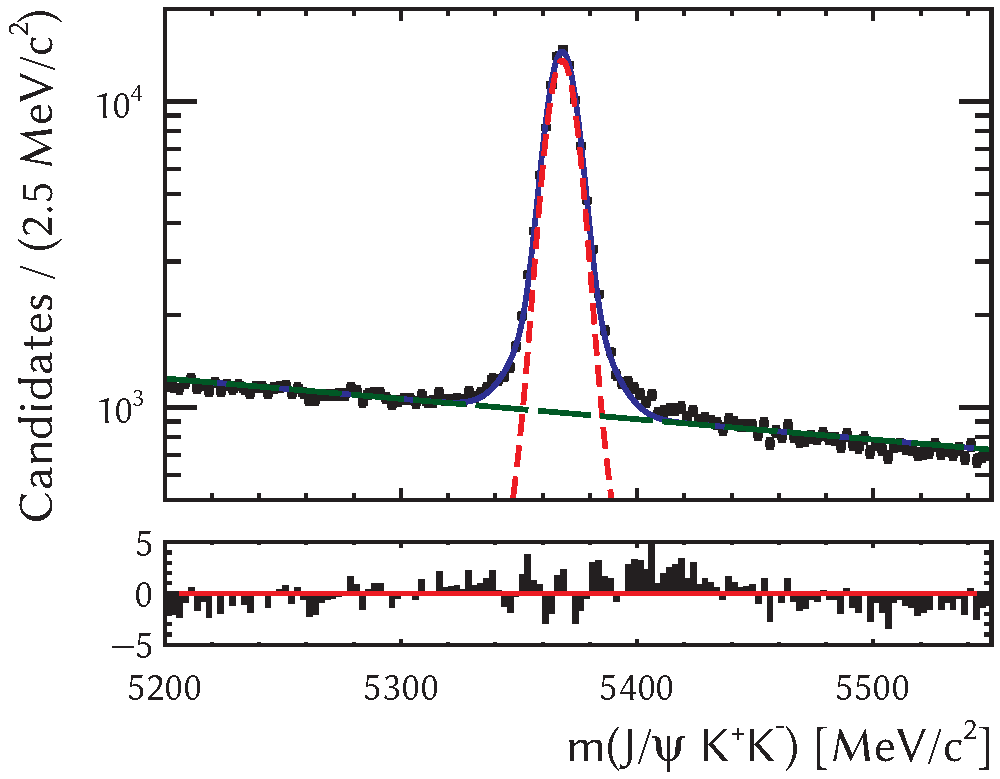
\includegraphics[width=\textwidth]{graphics/analysis/JpsiKKMass_DG_log_resid}
    \caption{}
    \label{fig:JpsiKKMass_DG_log}
  \end{subfigure}%
  \caption{Distribution of \BstoJpsiKK{} decay candidates in $\JpsiKK$ mass for
           (a) the signal mass range and
           (b) the full mass range on a logarithmic vertical scale.
           The black points show the distribution of the data and the blue, solid line shows a model that was fitted to the data.
           The model is the sum of two Gaussian shapes for the signal (shown by the red, short-dashed line)
           and an exponential shape for combinatorial background (shown by the green, long-dashed line).}
  \label{fig:JpsiKKMass_DG}
\end{figure}

The Ipatia function is defined by
\begin{equation}
  I \equiv
  \begin{cases}
    \frac{A}{(B + m-\mu)^{n_L}} \qquad\qquad\qquad\ \ \ \text{if}\ \ m - \mu < -a_L\,\sigma \\
    \frac{C}{(D + m-\mu)^{n_R}} \qquad\qquad\qquad\ \ \ \text{if}\ \ m - \mu > +a_R\,\sigma \\
    \left[(m-\mu)^{2} + \delta^{2}\right]^{\frac{1}{2} \lambda - \frac{1}{4}}\, e^{\beta (m-\mu)}\,
          K_{\lambda - \frac{1}{2}}\big(\alpha \sqrt{(m-\mu)^2 + \delta^2}\big) \\
          \qquad\qquad\qquad\qquad\qquad\quad\ \ \text{if}\ \ -a_L\,\sigma < m - \mu < +a_R\,\sigma \ ,
  \end{cases}
\end{equation}
where $m$ is the mass variable, $K_{\nu}(z)$ is the modified Bessel function of the second kind, the parameter $\delta$ is defined by
$\delta\equiv\sigma\sqrt{\frac{\zeta\,K_\lambda(\zeta)}{K_{\lambda+1}(\zeta)}}$, and $\alpha$ is defined by
$\alpha\equiv\frac{1}{\sigma}\sqrt{\frac{\zeta\, K_{\lambda+1}(\zeta)}{K_\lambda(\zeta)}}$. The parameter $\mu$ controls the position of
the mass peak, $\sigma$ and $\zeta$ control its width, and $\lambda$ controls its shape. The Ipatia function has an enhanced tail on both
the left and the right side, the positions and shapes of which are controlled by the parameters $a_{L/R}$ and $n_{L/R}$, respectively. The
parameter $\beta$ is fixed to zero and the parameters $A$, $B$, $C$, $D$ are obtained by imposing continuity and differentiability

\begin{figure}[htb]
  \centering
  \begin{subfigure}{0.49\textwidth}
    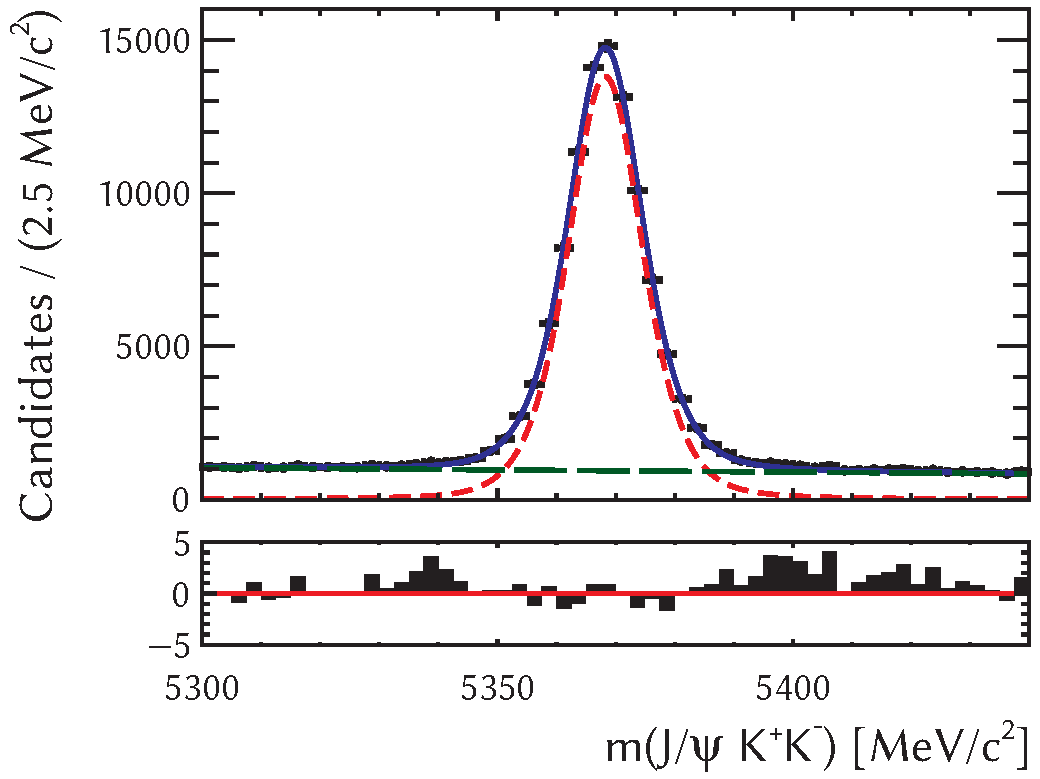
\includegraphics[width=\textwidth]{graphics/analysis/JpsiKKMass_I2_lin_resid}
    \caption{}
    \label{fig:JpsiKKMass_I2_lin}
  \end{subfigure}%
  \hfill%
  \begin{subfigure}{0.49\textwidth}
    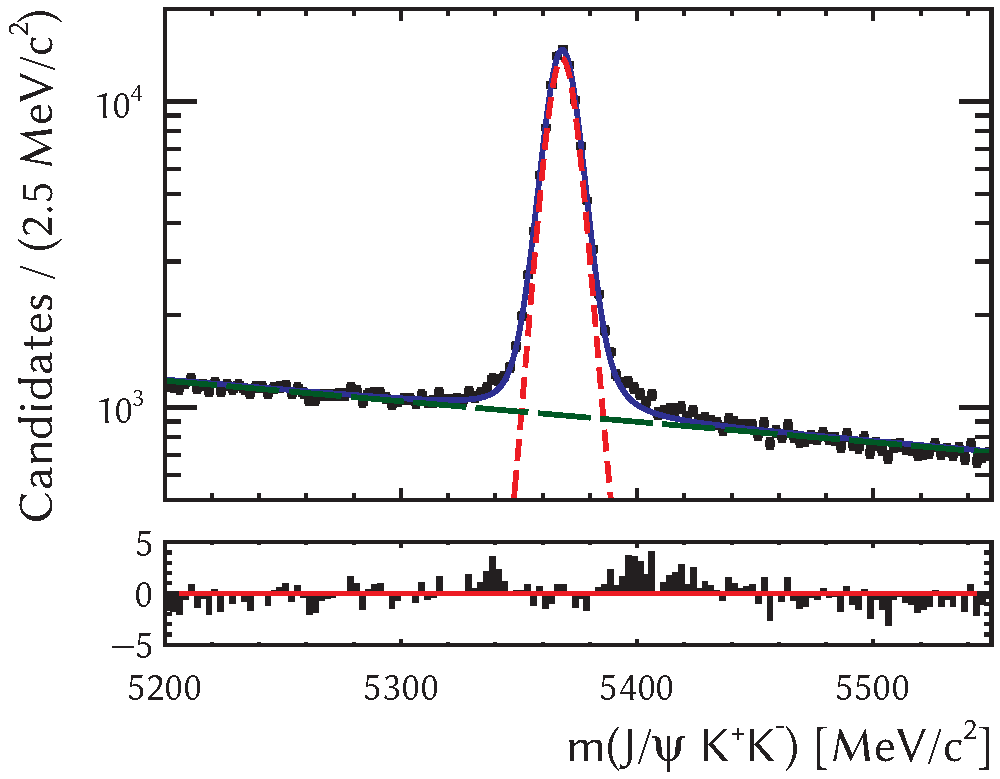
\includegraphics[width=\textwidth]{graphics/analysis/JpsiKKMass_I2_log_resid}
    \caption{}
    \label{fig:JpsiKKMass_I2_log}
  \end{subfigure}%
  \caption{Distribution of \BstoJpsiKK{} decay candidates in $\JpsiKK$ mass for
           (a) the signal mass range and
           (b) the full mass range on a logarithmic vertical scale.
           The black points show the distribution of the data and the blue, solid line shows a model that was fitted to the data.
           The model is the sum of an Ipatia shape for the signal (shown by the red, short-dashed line)
           and an exponential shape for combinatorial background (shown by the green, long-dashed line).}
  \label{fig:JpsiKKMass_I2}
\end{figure}

\begin{figure}[htb]
  \centering
  \begin{subfigure}{0.49\textwidth}
    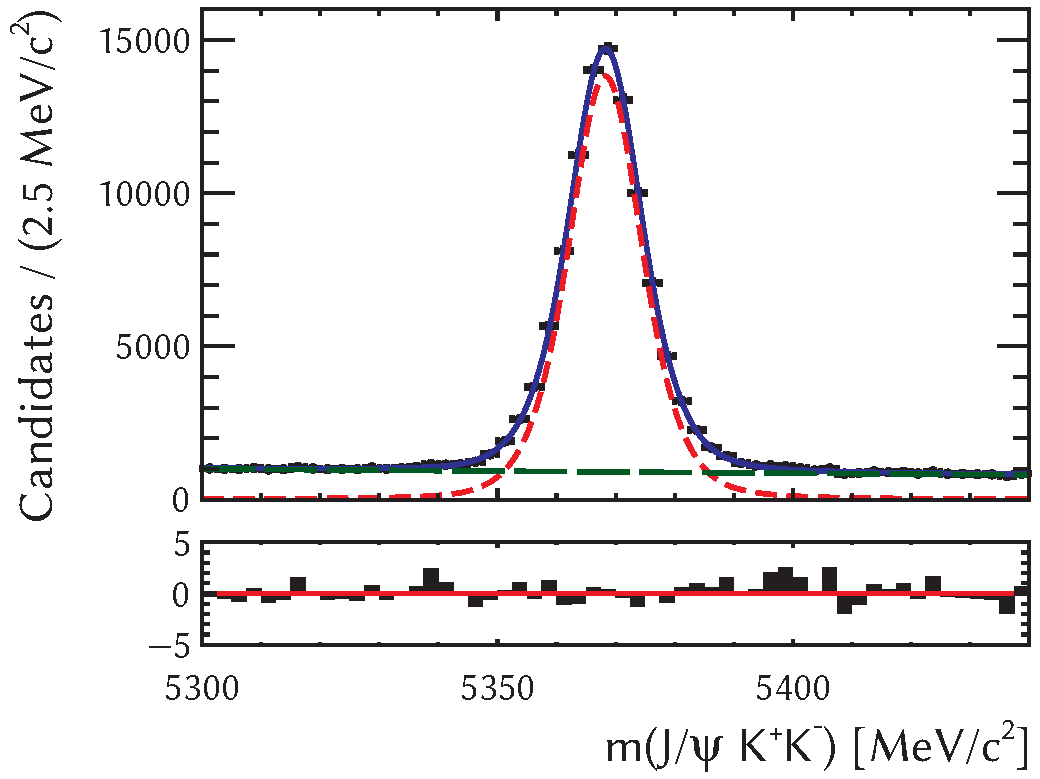
\includegraphics[width=\textwidth]{graphics/analysis/JpsiKKMass_I2_bkgSub_lin_resid}
    \caption{}
    \label{fig:JpsiKKMass_I2_bkgSub_lin}
  \end{subfigure}%
  \hfill%
  \begin{subfigure}{0.49\textwidth}
    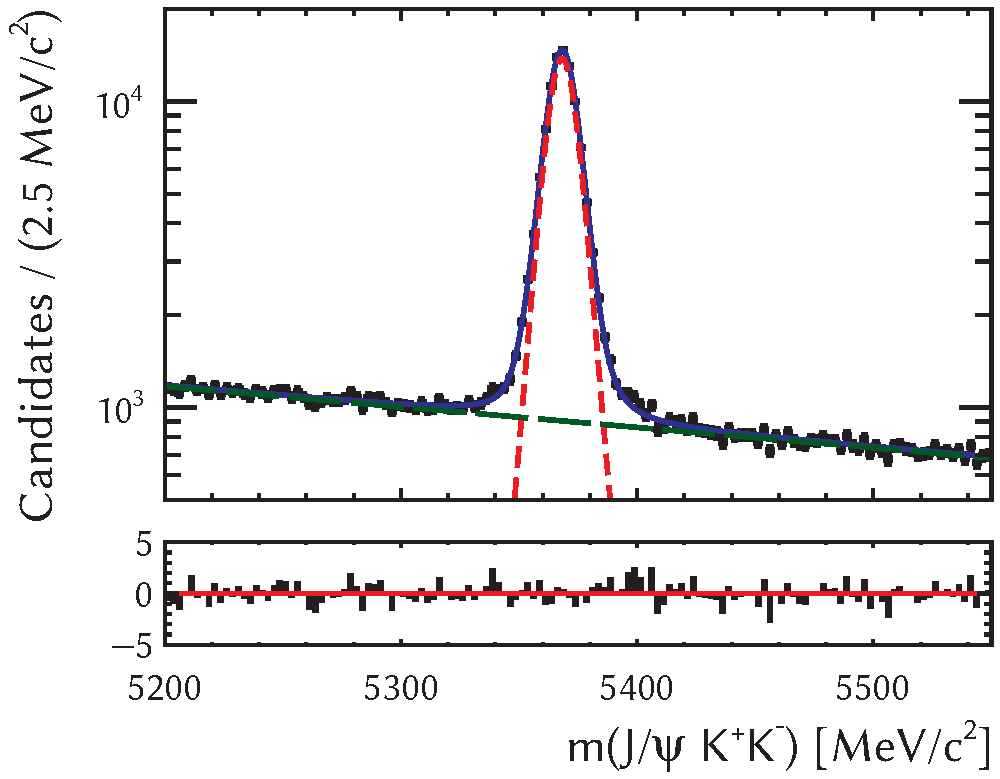
\includegraphics[width=\textwidth]{graphics/analysis/JpsiKKMass_I2_bkgSub_log_resid}
    \caption{}
    \label{fig:JpsiKKMass_I2_bkgSub_log}
  \end{subfigure}%
  \caption{Distribution of \BstoJpsiKK{} decay candidates in $\JpsiKK$ mass after subtracting resonant backgrounds for
           (a) the signal mass range and
           (b) the full mass range on a logarithmic vertical scale.
           The black points show the distribution of the data and the blue, solid line shows a model that was fitted to the data.
           The model is the sum of an Ipatia shape for the signal (shown by the red, short-dashed line)
           and an exponential shape for combinatorial background (shown by the green, long-dashed line).}
  \label{fig:JpsiKKMass_I2_bkgSub}
\end{figure}


\begin{figure}[htb]
  \centering
  \begin{subfigure}{0.49\textwidth}
    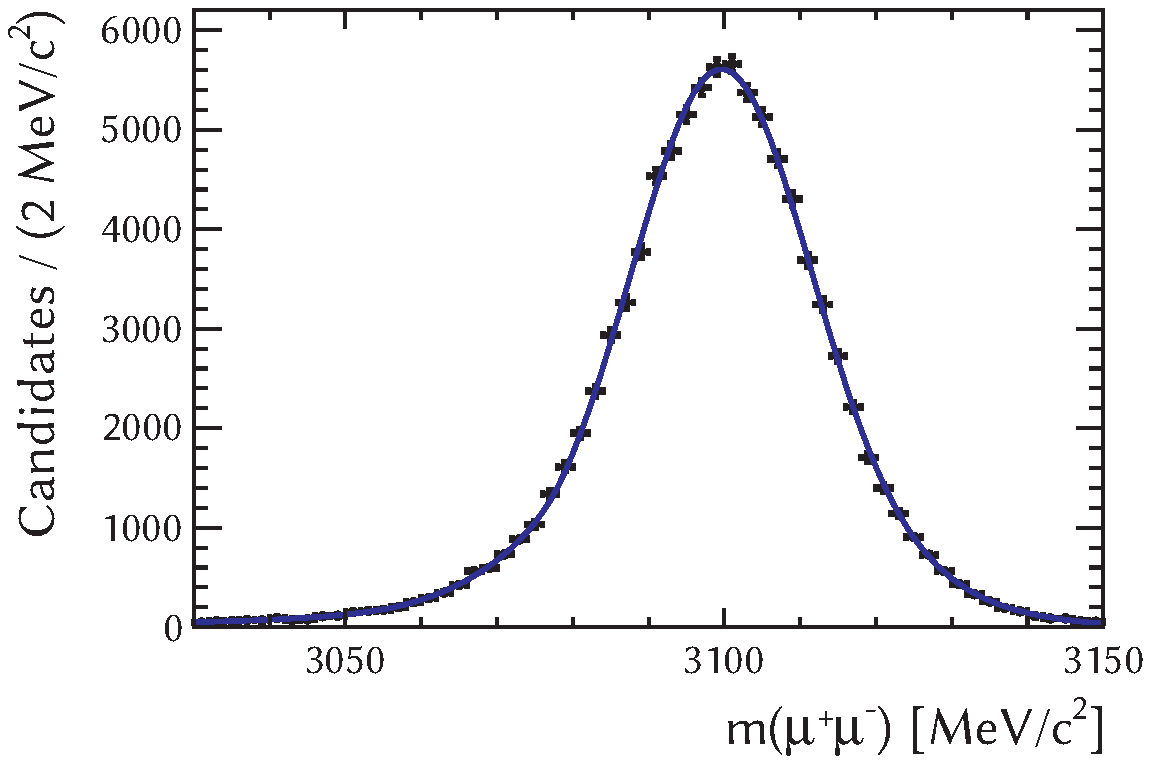
\includegraphics[width=\textwidth]{graphics/analysis/mumuMass}
    \caption{}
    \label{fig:mumuMass}
  \end{subfigure}%
  \hfill%
  \begin{subfigure}{0.49\textwidth}
    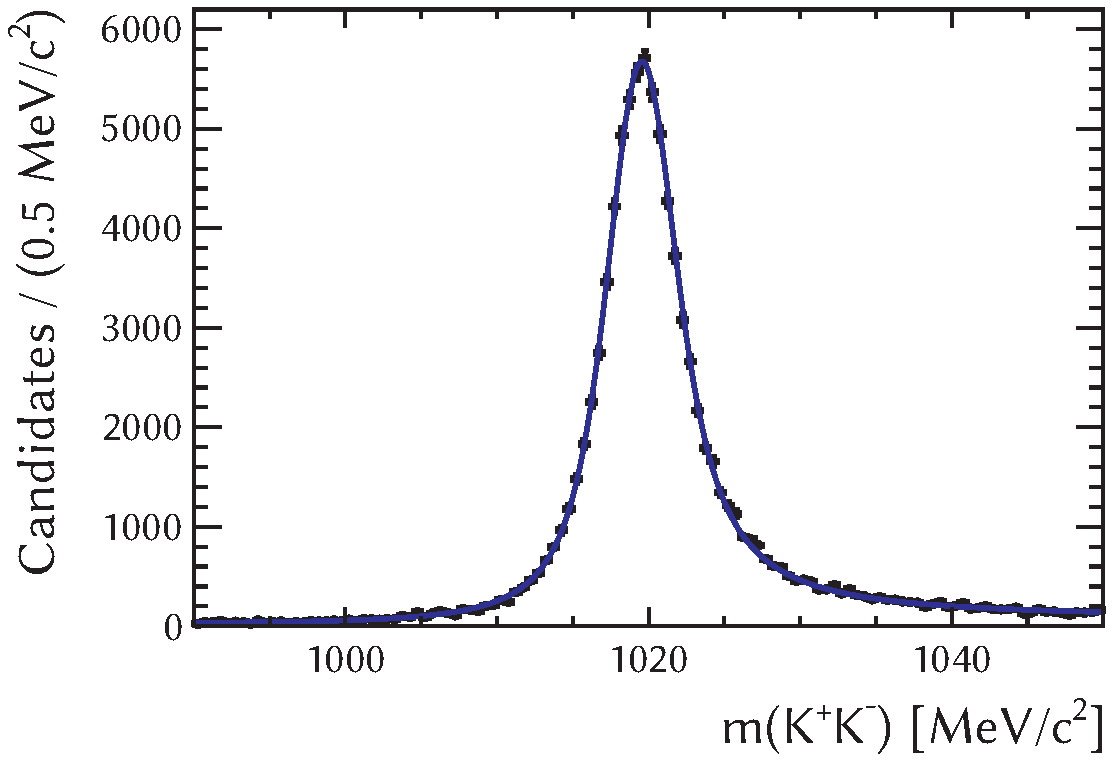
\includegraphics[width=\textwidth]{graphics/analysis/KKMass}
    \caption{}
    \label{fig:KKMass}
  \end{subfigure}%
  \caption{Background-subtracted distribution of \BstoJpsiKK{} decays in (a) $\mumu$ mass and (b) $\KK$ mass.}
  \label{fig:mumuKKMass}
\end{figure}
